
\section{Descriere}

TrustNews este aplicația care își propune să întregească toate elementele criptografice prezentate în teza de disertație pentru a crea o formă stabilă și sigură împotriva știrilor false. Ea își propune să acumuleze un număr mare de parteneri și cu timpul poate chiar să înlocuiască multitudinea de platforme pe care trusturile de știri publică informații.\\

Se dorește înlocuirea fundamentală a elementului clasic întâlnit în majoritatea platformelor de știri. Vorbesc despre bazele de date centralizate care salvează întreg conținutul într-un singur punct de control și de care depinde platforma de distribuire sub formă de website web.\\

Atacurile asupra website-urilor de acest tip pot avea la bază două scopuri ce vizează datele. Primul scop ar fi criptarea datelor printr-un atac ransomware iar al doilea ar consta în SQL Injection pentru a altera informația.
Acest al doilea scop este principalul vizat în contextul știrilor false și poate face ca o simplă modificare a unei propoziții să schimbe sensul întregului text.\\

Pentru a elimina aceste riscuri TrustNews se folosește de blockchain pentru a stoca știrile în structuri bine definite. Blockchain-ul prin natura lui implică o rețea în care sunt mulți participanți fiecare putând să contribuie cu noi informații. Un atacator nu mai poate acum acționa asupra unui singur punct de control și ar fi nevoit să acționează asupra întregii rețele iar asta ar implica să dețină o putere de procesare mare. De asemenea datele sunt acum salvate pe fiecare nod participant în rețea și fiecare informație are un posesor. În acest caz unui atacator îi este foarte greu să altereze informația chiar și din propria copie regăsită pe nodul pe care lucrează.\\

\clearpage

Fiecare nod va putea avea două roluri în aplicație. Primul este cel implicit și arată faptul că pe orice nod se va regasi o copie a întregului conținut salvat în blockchain dat de totalitatea știrilor. Al doilea rol este cel de extractor (scraper) de știri. Aplicația TrustNews își va prelua informația doar din surse de încredere, trusturi de știri cu o reputație crescută despre care putem să afirmăm că nu publică știri false.\\

Siguranța informației regăsită într-o sursă este în responsabilitatea celor care administrează respectivul website. TrustNews își propune astfel să fie pe lângă o zona mai eficientă din care să fie preluate știri și o formă de backup pentru totalul extras. Ea nu își propune să îmbunătățească securitatea website-urilor de unde extrage știri ci se bazează pe încrederea în trusturile alese.
Aplicația va scana constant mediile și va prelua de fiecare dată prima formă în care știrile au fost publicate. Odată salvată informația în blockchain avem garanția că textul este cel cu adevărat real. Un atacator care ar reuși să atace website-ul și să modifice știrile dându-le un nou sens nu ar putea efectua acest lucru la fel de ușor și în forma nouă.\\

Tehnologia BigchainDB este folosită pentru a acoperi cadrul blockchain. Aplicația TrustNews constă într-o rețea privată în care va exista întotdeauna o autoritate de control în care membrii participanți vor avea încredere. El este de regulă primul nod din rețea care distribuie software-ul aplicației și informațiile publice lui altor participanți. Este util să fie un context privat deoarece nu ne dorim un număr foarte mare de participanți și ne dorim totodată un factor de decizie mare asupra a ce trebuie să se facă când cineva încalcă anumite reguli. De asemenea cadrul privat reduce nevoia alocării unei cantități de resurse mari pentru a desfășura procesele din algoritmul blockchain.\\

BigchainDB permite în ultimele versiuni ale software-ului tranzacții specifice de tip votare (election). Cu acestea se pot adăuga ușor membri noi în rețeaua blockchain. Tranzacțiile vor ajunge ca oricare alta la fiecare nod din rețea existent până în acel punct și fiecare va putea lua o decizie în algoritmul de consens. În acest mod putem fi siguri că fiecare nod cunoaște toate celelalte noduri.\\

O proprietate importantă a aplicației este că își extrage știrile dintr-o varietate foarte mare de platforme. Acest lucru este util din punctul de vedere al conținutului deoarece se salvează informații din toate domeniile dar și din punct de vedere al securității. Lista de platforme trebuie să fie publică pentru a crea un grad sporit de încredere cu cei ce citesc demonstrând că datele sunt luate de pe platforme cu o reputație crescută. De asemenea pentru ca un atacator să poată influența conținutul știrilor din blockchain ar însemna să reușească să treacă de mecanismele de securitate a unui număr mare de website-uri.\\

\clearpage

Cu toate că lista totală de surse este publică, nu este obligatoriu nevoie ca fiecărei știri salvată în blockchain să i se eticheteze și sursa de unde provine. Un atacator s-ar putea închipui ca un nod corect pentru a avea acces la procesul de tranzacționare și ar putea urmări pasiv ce conținut se extrage și de unde. Astfel el ar putea să își creeze surse de atac reprezentând platformele de interes pentru el, cu intenția de a adăuga știri contrafăcute știind că extractorul la un moment dat va ajunge să preia informația falsă.\\

Pentru a masca și totodată verifica sursa vom folosi structurile de dovedire de tip zkSNARKs. Conversia către un context matematic se poate face prin alocarea un număr prim diferit fiecărei platforme. În acest fel un nod extractor va trebui să calculeze produsul tuturor valorilor și va trebui să demonstreze că numărul prim asociat platformei de pe care a extras știrea divide produsul, fără a-l expune.\\

Pentru a extrage știrile aplicația TrustNews poate fi configurată să folosească orice utilitar de tip scraper. Acesta va fi responsabil de navigarea către anumite puncte pe website cât și de preluarea textului știrilor din conținutul HTML. 

Având forma prin care se extrage textul unei știri și forma prin care se ascunde sursa de unde este preluată informația se poate acum lărgi structura unei tranzacții din blockchain. Fiecare tranzacție va avea acum câmpul de date compus din patru elemente titlul știrii, textul știrii, dovada sursei și momentul de timp când se creează. \\

\clearpage

\section{Modul de funcționare}

TrustNews este construită folosind limbajul de programare NodeJS pentru a putea integra ușor totalul de tehnologii folosite în aplicație. Totuși se poate converti la alt limbaj de programare dacă există module similare scrise în noul limbaj ales. Python este un astfel de exemplu ce permite utilizarea unor module similare pentru ca aplicația să aibă același comportament. \\

Funcția principală a aplicației numită \textit{Main()} \cite{TrustNews_Main} este cea în care se programează extragerile de știri regulate la un interval de secunde ales de noi. Se poate seta în funcție de preferință un interval de 30 de secunde pentru a extrage cu o viteză foarte mare sau un interval de chiar câteva ore pentru a încetini fluxul.\\

Funcția care face extragerea propriu-zisă este \textit{Extract()} \cite{TrustNews_Extract} și cuprinde un plan bine definit de apelări de funcții din librării standard folosite pentru a interacționa cu tehnologiile alese.\\

În primul rând se folosește de structura publică ce mapează fiecare platformă de știri de un număr prim diferit. Pentru un exemplu restrâns am ales să folosesc
\begin{verbatim}
var news_platforms = [
  { name: "CNN", prime_nr: "3" },
  { name: "BBC", prime_nr: "5" },
  { name: "The Economist", prime_nr: "7" },
  { name: "The Wall Street Journal", prime_nr: "11" },
  { name: "World Health Organization", prime_nr: "17" },
];
\end{verbatim}
, însă într-un context real această mapare poate conține zeci de astfel de perechi.

Aplicația, la fiecare iterație, va calcula produsul tuturor numerelor prime și va alege la întâmplare o sursă din mulțimea dată.\\

În funcție de sursa aleasă se merge mai departe în etapa de parsare/scraping a conținutului HTML de pe website-ul asociat platformei de știri. Pentru scraping am folosit utilitarul \textit{scraperjs} \cite{scraperjs} ce ușurează mult procesul având nevoie doar de identificatorii HTML pentru a ști la ce elemente să se uite. Se folosește un scraper static pentru a putea iniția un lanț de promisiuni de tip Javascript, cu alte cuvinte promisiuni că procese noi vor fi create și vor rula în paralel pentru a extrage conținutul de care avem nevoie din pagini.\\

Cu ajutorul lui extragem titlul și conținutul știrii pe care le întoarcem în funcția de extragere de la care am plecat.\\

\clearpage

În continuare se construiește structura de dovedire ce atestă că sursa știrii este una folosită în cadrul aplicației TrustNews. Am folosit utilitarul \textit{ZoKrates} \cite{zokrates} pentru a putea crea întregul sistem ce conține atât etapa inițială de configurare cât și etapele ulterioare de creare a dovezilor și de verificare a lor.\\

În primul rând se consideră etapa de configurare deja efectuată de către nodul supervizor asupra întregii rețele blockchain. El va scrie codul programul cu care se vor putea crea dovezi, îl va compila și va crea pe baza lui CRS-ul, cunoscut și ca perechea de chei pentru dovedire și pentru verificare. Toate aceste trei etape vor fi efectuate o singură dată iar la finalul lor nodul supervizor este responsabil să publice în cadrul rețelei toate valorile calculate.\\

Compilatorul ZoKrates lucrează cu programe scrise într-un limbaj propriu de nivel înalt foarte asemanator cu Python. Codul conține verificarea logică că parametrul public reprezentat de produsul numerelor prime divide parametrul păstrat secret (witness) reprezentat de numarul prim asociat sursei de unde a fost extrasă știrea precedentă.
\begin{verbatim}
def main(private u32 chosen_site_prime_nr, u32 product_of_primes) -> bool:
    return product_of_primes % chosen_site_prime_nr == 0
\end{verbatim}

Pentru a genera o dovadă folosim funcția \textit{GenerateProof(witness)} \cite{TrustNews_GenerateProof} care va primi sub formă de șir de caractere valorile parametrilor din funcție. El se va folosi la bază de două dintre apelurile utilitarului, \textit{compute-witness} pentru a genera o structură binară a valorilor cunoscute de doveditor și \textit{generate-proof} pentru a construi fișierul dovadă în format JSON având ca argumente fișierul binar generat de comanda precedentă și cheia de dovedire cunoscută public.\\

Pentru verificare se poate folosi funcția \textit{VerifyProof(proof)} \cite{TrustNews_VerifyProof} care va primi ca argumente fișierul dovadă, va prelua cheia de verificare publică și va întoarce rezultatul "PASSED" dacă verificarea se realizează cu succes.\\

Având cele trei elemente deja preconstruite, titlu, conținut și dovadă, funcția poate continua la asamblarea tranzacției care le va curpinde pe toate.\\

În primul rând se presupune că fiecare nod în momentul în care intră în rețeaua aplicației TrustNews își va genera o pereche de chei criptografice pe care le va folosi la crearea și semnarea tranzacțiilor. Se poate folosi codul \textit{GenerateNodeKeys.js} \cite{TrustNews_GenerateNodeKeys} pentru generarea unui fișier ce conține perechea necesară.\\

\clearpage

Tranzacția realizată folosind utilitarul scris în Javascript pentru BigchainDB va fi de tip CREATE, va fi creată folosind funcția \textit{CreateNews()} \cite{TrustNews_CreateNews} și va avea ca parametri cele trei elemente generate de funcțiile precedente și perechea de chei. Câmpul de date marcat ca asset va conține structura 
\begin{verbatim}
var asset = {
    title: title,
    content: content_of_news,
    proof: proof,
    datetime: new Date().toString(),
};
\end{verbatim}\\

Nodul care va crea tranzacția va fi și cel carui îi va aparține știrea extrasă, de aceea cheia publică va fi folosită atât la câmpul issuers cât și la outputs. După ce tranzacția este semnată folosind cheia privată, este transmisă în rețeaua blockchain și un mesaj de tip "CREATE Transaction successfully posted." va fi afișat după ce își va termina ciclul de validare.\\

Pentru o dezvoltare în timp a aplicației a fost implementată și funcția \textit{TransferNews()} \cite{TrustNews_TransferNews}. Spre deosebire de funcția de creare, aceasta va primi ca parametru direct structura pentru input-uri conținând referințele către tranzacții deja procesate. Cheile folosite vor fi cea publică a nodului care va intra în posesia știrii și cea privată a actualului deținător pentru a dovedi că întradevar le poate accesa.\\

Ultimul pas din funcția de extagere este dat de afișarea conținutului din știre. Verificarea că o tranzacție a fost adaugată în blockchain se face folosind funcția \textit{CheckTransaction(transaction\_id)} \cite{TrustNews_CheckTransaction} care apelează API-ul "/api/v1/transactions/\$\{transaction\_id\}" și întoarce întregul conținut al tranzacției.\\

\clearpage

\section{Exemplu de funcționare}

Pentru testare am folosit un sistem de operare Ubuntu 18.04 având instalate Docker, NodeJS, ZoKrates CLI, npm și toate modulele asociate aplicației: scraperjs, child\_process, axios, bigchaindb-driver, fs, util. Pentru BigchainDB am folosit un container cu imaginea de tip all-in-one.

În exemplul următor preiau o știre de pe platforma online BBC.com. Pe pagina principală regăsesc toate titlurile și toate URL-urile către paginile actualelor știri. Aleg o pereche la întâmplare și preiau conținutul text folosind o nouă instanță de scraper pentru URL-ul știrii alese.

\begin{figure}[H]
    \centering
    \subfloat[]{{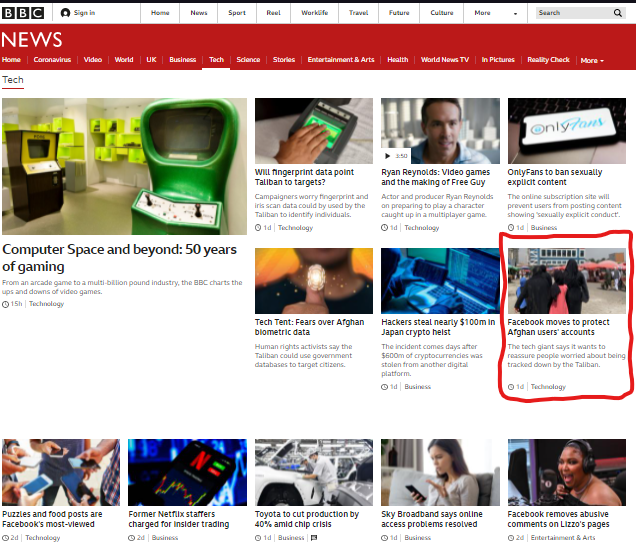
\includegraphics[scale=0.50]{Images/SCR1.png}}}
    \qquad
    \subfloat[]{{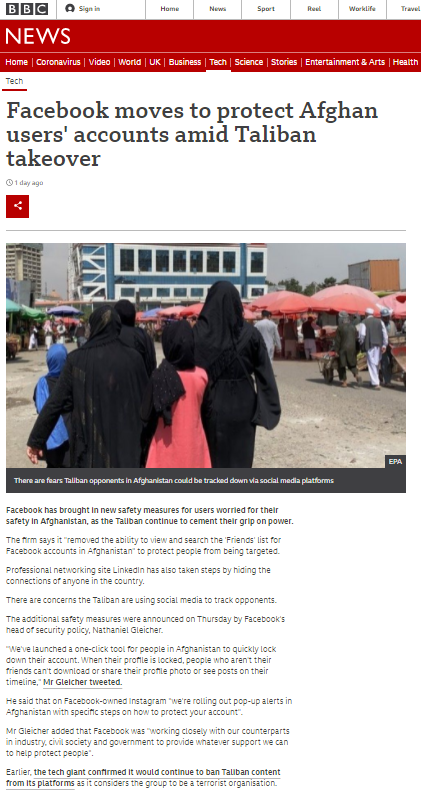
\includegraphics[scale=0.35]{Images/SCR2.png}}}
    \caption{Știre de pe website-ul oficial - sursă \cite{BBC}}
\end{figure}

\begin{figure}[H] 
\centering
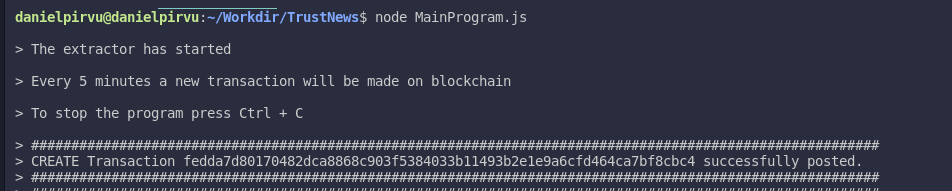
\includegraphics[scale=0.6]{Images/SCR3.png}
\caption{Output după procesarea tranzacției}
\end{figure} 

\clearpage

Procesul de dovedire se folosește de convenția stabilită că fiecare platformă de știri are asociat numărul prim. Website-ul BBC.com are asociat numărul 5 iar produsul calculat pe baza tuturor asocierilor este 19635 = 3 * 5 * 7 * 11 * 17. În dovadă se văd doar constantele folosite pentru a arata că se cunosc polinoamele implicate în QAP de către doveditor datorită valorii witness. Valorile de input publice vor fi de asemenea regăsite în dovadă. În cazul acesta, valoarea 0x4cb3, reprezentând produsul total în valoare hexazecimală, este prezentă.\\

\begin{figure}[H] 
\centering
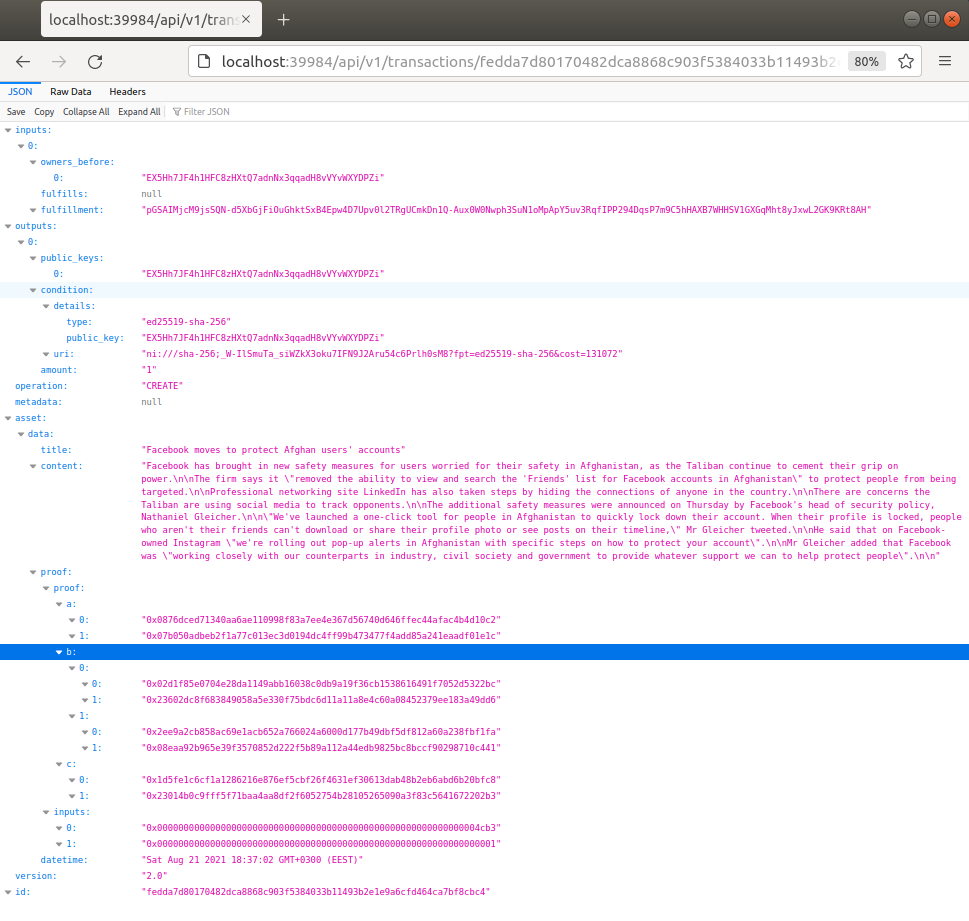
\includegraphics[scale=0.65]{Images/TN_Full_Create.png}
\caption{Tranzacție de tip CREATE pentru TrustNews}
\end{figure}

\clearpage

\section{Planuri de îmbunătățire}

În final, fiecare nod va ajunge să conțină o cantitate mare de știri preluate din foarte multe surse diferite. O primă îmbunătățire ar putea consta în expunerea știrilor pe o platforma nouă administrată tot în cadrul rețelei blockchain. Practic un nod va juca și rolul de server web unde vor putea fi citite știrile.\\

În continuarea acestei idei fiecare nod extractor va putea tranfera știrea creată către nodul ales pentru a fi server web. Acesta din urmă va putea interoga ușor toate output-urile din toate tranzacțiile ce au cheia lui publică specificată. Astfel va putea obține id-urile tranzacțiilor și poate ajunge la conținutul știrii din interior.\\

Aplicația am văzut că tratează cazul în care nodurile pot fi deținute de oricine primește acces în rețeaua privată. Odată ce un nod este prezent el poate să extragă informații de pe platforme deja existente și unde publicarea se face de către persoane autorizate. Pentru a îmbunătăți performanță aplicației se poate implementa o formă simplificată de nod care va fi deținută de trusturile de media care ar putea salva direct în blockchain conținutul nou.\\

Fiecare trust va fi restricționat să dețină un singur nod cu care va putea adăuga conținut. În continuare ar putea fi implementat un sistem de votare prin care celelalte trusturi și-ar putea exprima opinia despre câtă încredere le acordă. Fiecare știre va avea astfel un rating asociat și fiecare cititor va putea interpreta pe baza lui dacă o știre este falsă.\\

Mulțimea mare de surse poate ridica problema drepturilor de autor. Trebuie astfel să fie structurat un plan prin care fiecărui trust îi este comunicată activitatea aplicației. Discutând cu trusturile de publicitate, aplicația poate evolua spre una din ideile menționate anterior sau poate extrage altele noi.\\

Mai rămâne în picioare problema știrilor duplicat. Fiecare nod va trebui să mențină o proprie listă a știrilor pe care deja le-a extras cât și o listă cu știri pe care alte noduri le-au procesat. Acest din urmă aspect este greu de realizat deoarece nodurile funcționează în paralel și nu comunica decât în momentul în care au creat deja tranzacțiile. Comparând două tranzacții cu același text al știrii vom vedea că sunt multe elemente ce le disting precum cheile criptografice, momentul de timp și chiar și dovezile.\\

O altă formă de duplicat ține de natura semantică a informației. Știm că o informație poate să fie publicată pe două sau mai mai multe platforme toate fiind de încredere. Pentru că titlurile și nuanța cuvintelor poate fi diferită de la o platforma la altă ar fi nevoie de un modul de inteligență artificială care ar putea calcula un grad de similitudine, valoare după care putem decide dacă două știri sunt identice sau nu.\\